\documentclass[fleqn, 10pt]{article}

% Paquetes necesarios
\usepackage[utf8]{inputenc}
\usepackage{graphicx} 
\usepackage{amsthm, amsmath}
\usepackage{nccmath} %Para centrar ecuaciones
\usepackage{graphicx}
\usepackage{enumitem}

% Personalizo mi alfabeto
\DeclareMathAlphabet{\pazocal}{OMS}{zplm}{m}{n}
\newcommand{\Lb}{\pazocal{L}}

% Definimos los entornos para definiciones, teoremas, etc...
\theoremstyle{plain}
\newtheorem{proposicion}{Proposición}

\theoremstyle{definition}
\newtheorem{definition}{Definición}[section]
\newtheorem{example}{Ejemplo}[section]

%Definimos el título
\title{Teoría de Autómatas y Lenguajes Formales\\[.4\baselineskip]Práctica 3}
\author{José Manuel Rodríguez Chicano}
\date{\today}

%Comienzo del documento
\begin{document}

%Generamos el título
\maketitle

\section{Ejercicio 1}

Define the TM solution of exercise 3.4 of the problem list and test its correct
behaviour.

La maquina de Turing sería la siguiente.
\begin{center}
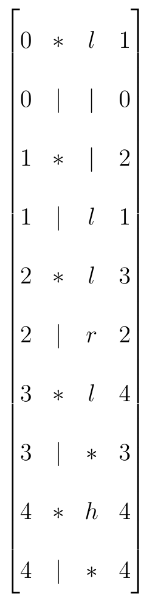
\includegraphics[width=3cm, height=10cm]{Turing.png}
\end{center}
Y su resolución en JFLAP (de manera invertida porque en este comienza a la izquierda en vez de a la derecha) Sería la siguiente.
\begin{center}
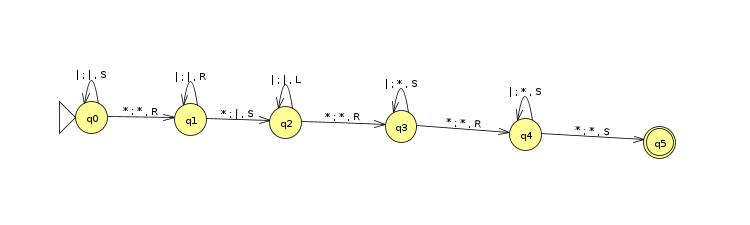
\includegraphics[width=15cm, height=6cm]{JFLAP.png}
\end{center}
Esta máquina de Turing ha sido comprobada con éxito, la probé con 1 + 1, es decir $||*||$ al ser unaria y con $|||*||$ es decir 2+1 y los resultados fueron los esperados, es decir $|||$ y $||||$
\section{Ejercicio 2}

Define a recursive function for the sum of three values.
\\

En este caso utilizamos la recursion primitiva que viene definida en los apuntes de la siguiente manera:

Let $k\geq 0$ and the functions
\\
$g:{N}^k -> {N}$
\\
$h:{N}^{k+2} -> {N}$
\\
$f:{N}^{k+1}  ->  {N}$ 


\begin{center}
    $f(\vec{n},m)=\left\{ 
\begin{array}{lcc}
    g(\vec{n})                          & \text{if} & m=0\\
    h(\vec{n},m-1,f(\vec{n},m-1)) & \text{if} & m>0 
\end{array}\right.$
\end{center}

Entonces la definición de la función recursiva para la suma de 3 que he implementado es la siguiente:
\\
\\
$addition3(n)= <<\pi^1_1 | \sigma(\pi^3_3) | \sigma(\pi^4_4)> (n)$
\\
\\
Probando así en octave con los ejemplos 3+3+5 cuyo resultado es 11:
\begin{center}
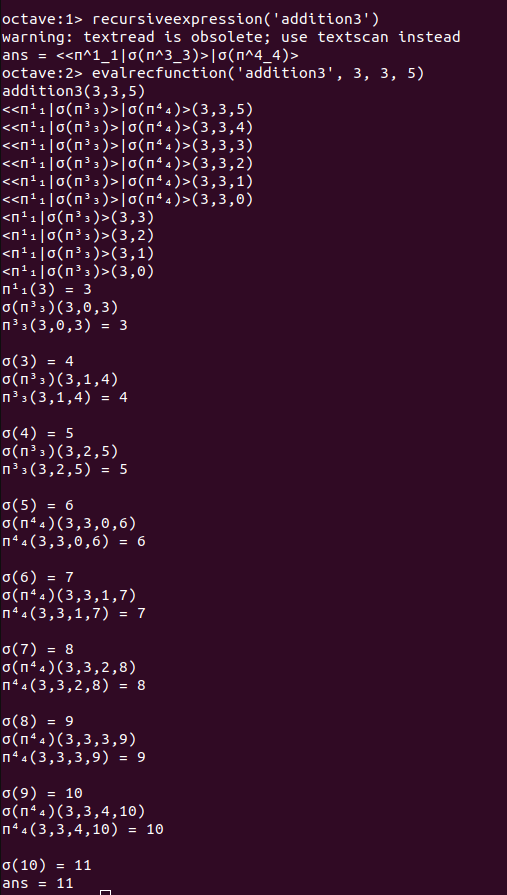
\includegraphics[width=5cm, height=10cm]{2.png}
\end{center}
\section{Ejercicio 3}
Implement a WHILE program that computes the sum of three values. You
must use an auxiliary variable that accumulates the result of the sum.

\begin{center}
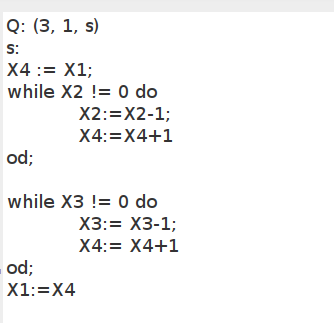
\includegraphics[width=7cm, height=6cm]{3.png}
\end{center}
\end{document}